\documentclass[11pt]{article}

% ---------- packages ----------
\usepackage[utf8]{inputenc}
\usepackage[T1]{fontenc}
\usepackage[margin=1in]{geometry}
\usepackage{amsmath,amssymb}
\usepackage{graphicx}
\usepackage{booktabs}
\usepackage{array}
\usepackage{caption}
\usepackage{xcolor}
\usepackage{enumitem}
\usepackage{listings}
\usepackage{tikz}
\usetikzlibrary{positioning,arrows.meta,fit}
\usepackage[section]{placeins} % keep floats inside their section (no drift into References)
\usepackage[colorlinks=true,linkcolor=blue,urlcolor=blue,citecolor=blue]{hyperref}

% figures live in the repo under this path (works with Overleaf GitHub sync)
\graphicspath{{stage2/results/figures/}{./}}

% compact code style for the reproduce appendix
\definecolor{codebg}{gray}{0.96}
\lstset{
  basicstyle=\ttfamily\small,
  backgroundcolor=\color{codebg},
  breaklines=true,
  columns=fullflexible,
  frame=single,
  framesep=4pt,
  xleftmargin=4pt,
  aboveskip=6pt,belowskip=6pt,
  literate={±}{{$\pm$}}1 {×}{{$\times$}}1 {→}{{$\rightarrow$}}1
}

\newcommand{\code}[1]{\texttt{#1}}

% ---------- title ----------
\title{\textbf{CovidGAN --- Paper Reconstruction and Improvement}\\[4pt]
\large Final Project, Part 2}
\author{}
\date{}

\begin{document}
\maketitle
\vspace{-2.5em}

\noindent
Reconstruction and improvement of Waheed, Goyal, Gupta, Khanna, Al-Turjman,
Pinheiro, \emph{``CovidGAN: Data Augmentation Using Auxiliary Classifier GAN for
Improved Covid-19 Detection''}, IEEE Access, vol.~8, 2020.

\medskip
\noindent
This is the \textbf{unified report} for both stages. \textbf{Stage~1} reconstructs
the paper's AC-GAN + VGG16 COVID-19 detector; \textbf{Stage~2} improves the
architecture and shows the effect in a paper\,/\,reconstruction\,/\,improved table.
A large part of the work was \textbf{experimental investigation}: our
reconstruction did \emph{not} match the paper on two points --- our baseline came
out higher than the paper's, and GAN augmentation came out flat rather than +10 ---
and most of Stage~1 is a sequence of controlled tests that try to explain why.
Those tests motivated the Stage~2 design, which does recover a positive
augmentation lift. Throughout, we treat these tests as \emph{support for or against}
a hypothesis, not as proof.
It follows the required structure (Original architecture, Paper results,
Reconstruction results, Improved architecture, Improved results, Discussion,
References), with a short reproduce-commands section just before the references.
Numbers behind every table live in \code{stage2/results/}.

\tableofcontents
\bigskip

% =====================================================================
\section{Original architecture}
% =====================================================================

The paper's pipeline has two models: an \textbf{AC-GAN} that synthesizes
chest-X-ray (CXR) images, and a \textbf{VGG16-based classifier} that detects
COVID-19. Synthetic images from the GAN augment the classifier's training set.

Figure~\ref{fig:arch} sketches the three components at a block level; the exact
layer-by-layer specification (with parameter counts and source lines) is in
Table~\ref{tab:faithful}.

\begin{figure}[htbp]
\centering
% ---- shared node styles ----
\tikzset{
  b/.style={draw,rounded corners,minimum height=8mm,minimum width=15mm,font=\scriptsize,align=center,fill=blue!8},
  io/.style={draw,rounded corners,minimum height=8mm,minimum width=13mm,font=\scriptsize,align=center,fill=black!8},
  frz/.style={draw,rounded corners,minimum height=8mm,minimum width=15mm,font=\scriptsize,align=center,fill=black!18},
}

% ---- (a) Generator ----
\textbf{(a) AC-GAN generator}\\[2pt]
\resizebox{\textwidth}{!}{%
\begin{tikzpicture}[>=Latex,node distance=5mm and 7mm]
  \node[io] (z) {noise $z$\\$\mathbb{R}^{100}$};
  \node[io,below=of z] (c) {label $c$};
  \node[b,right=of z] (zd) {Dense+ReLU\\$7{\times}7{\times}1024$};
  \node[b,right=of c] (cd) {Embed$\to$Dense\\$7{\times}7{\times}1$};
  \node[b,right=8mm of zd] (cat) {concat\\$7{\times}7{\times}1025$};
  \node[b,right=of cat] (u1) {TConv$\uparrow$\\$14^2$};
  \node[b,right=of u1] (u2) {TConv$\uparrow$\\$28^2$};
  \node[b,right=of u2] (u3) {TConv$\uparrow$\\$56^2$};
  \node[b,right=of u3] (u4) {TConv+tanh\\$112^2$};
  \node[io,right=of u4] (img) {image\\$112{\times}112{\times}3$};
  \draw[->] (z) -- (zd); \draw[->] (c) -- (cd);
  \draw[->] (zd) -- (cat); \draw[->] (cd) -- (cat);
  \draw[->] (cat) -- (u1); \draw[->] (u1) -- (u2); \draw[->] (u2) -- (u3);
  \draw[->] (u3) -- (u4); \draw[->] (u4) -- (img);
\end{tikzpicture}}\\[10pt]

% ---- (b) Discriminator ----
\textbf{(b) AC-GAN discriminator}\\[2pt]
\resizebox{\textwidth}{!}{%
\begin{tikzpicture}[>=Latex,node distance=5mm and 7mm]
  \node[io] (img) {image\\$112^2{\times}3$};
  \node[b,right=of img] (d1) {Conv$\downarrow$};
  \node[b,right=of d1] (d2) {Conv$\downarrow$};
  \node[b,right=of d2] (d3) {Conv$\downarrow$};
  \node[b,right=of d3] (d4) {Conv$\downarrow$};
  \node[b,right=of d4] (d5) {Conv$\downarrow$\\$7{\times}7{\times}512$};
  \node[b,above right=3mm and 9mm of d5,fill=green!10] (val) {validity head\\(real / fake)};
  \node[b,below right=3mm and 9mm of d5,fill=orange!12] (cls) {class head\\(COVID / Normal)};
  \draw[->] (img) -- (d1); \draw[->] (d1) -- (d2); \draw[->] (d2) -- (d3);
  \draw[->] (d3) -- (d4); \draw[->] (d4) -- (d5);
  \draw[->] (d5) -- (val); \draw[->] (d5) -- (cls);
\end{tikzpicture}}\\[10pt]

% ---- (c) Classifier ----
\textbf{(c) VGG16 detector (classifier)}\\[2pt]
\resizebox{0.92\textwidth}{!}{%
\begin{tikzpicture}[>=Latex,node distance=5mm and 7mm]
  \node[io] (img) {image\\$112^2{\times}3$};
  \node[frz,right=of img] (vgg) {VGG16 conv base\\\textit{frozen} (ImageNet)};
  \node[b,right=of vgg] (gap) {GlobalAvg\\Pool};
  \node[b,right=of gap] (d64) {Dense(64)\\ReLU, Dropout};
  \node[b,right=of d64] (d2) {Dense(2)\\softmax};
  \node[io,right=of d2] (out) {COVID /\\Normal};
  \draw[->] (img) -- (vgg); \draw[->] (vgg) -- (gap); \draw[->] (gap) -- (d64);
  \draw[->] (d64) -- (d2); \draw[->] (d2) -- (out);
\end{tikzpicture}}
\caption{Block view of the three models. \textbf{(a)}~The generator fuses a noise
vector and a class label, then upsamples $7{\to}112$ through four transpose-conv
blocks ($\sim$22M params). \textbf{(b)}~The discriminator downsamples an image to
$7{\times}7{\times}512$ and splits into the two AC-GAN heads --- validity and class
($\sim$2M params). \textbf{(c)}~The detector is a \emph{frozen} ImageNet VGG16 base
with a small trainable head; only $\sim$33K of $\sim$14.7M params train (grey =
frozen).}
\label{fig:arch}
\end{figure}

\paragraph{Generator.} Inputs are a class label $c \in \{\text{COVID},
\text{Normal}\}$ and a noise vector $z \in \mathbb{R}^{100}$ ($z \sim
\mathcal{N}(0,0.02)$, per the paper). A label branch (Embedding$\to$Dense) and a
noise branch (Dense$\to$ReLU) are concatenated to $7{\times}7{\times}1025$ and
upsampled by four $5{\times}5$ stride-2 transpose-conv blocks (BatchNorm+ReLU,
$\tanh$ on the last) to a $112{\times}112{\times}3$ image in $[-1,1]$. ($\sim$22M
params.)

\paragraph{Discriminator.} Five $3{\times}3$ conv blocks (BatchNorm /
LeakyReLU(0.2) / Dropout(0.5)) downsample the image to $7{\times}7{\times}512$,
which feeds \textbf{two heads} --- a validity head (real/fake) and a class head
(COVID/Normal). The class head is what makes this an \emph{auxiliary-classifier}
GAN. ($\sim$2M params.)

\paragraph{Classifier (\code{build\_classifier}).} A \textbf{frozen} ImageNet
VGG16 convolutional base feeds GlobalAveragePool $\to$ Dense(64,\,ReLU) $\to$
Dropout(0.5) $\to$ Dense(2). Only the head trains ($\sim$33K params); the VGG16
base is frozen, matching the paper: \emph{``\ldots setting the `trainable'
property on each of the VGG layers to False before training.''}

\subsection{Losses / objective}
\begin{itemize}[nosep,leftmargin=1.4em]
  \item \textbf{GAN:} \code{BCEWithLogits} on the validity head +
        \code{CrossEntropy} on the class head, for both $D$ and $G$ (standard
        AC-GAN objective). One-sided label smoothing (real target 0.9).
  \item \textbf{Classifier:} \code{CrossEntropy}.
\end{itemize}

\subsection{Key hyperparameters (paper's)}
\begin{itemize}[nosep,leftmargin=1.4em]
  \item GAN: batch 64, Adam $\text{lr}=2\mathrm{e}{-4}$, $\beta_1=0.5$,
        \textbf{2000 epochs}.
  \item Classifier: batch 16, Adam $\text{lr}=1\mathrm{e}{-3}$, image size
        $112{\times}112$, pixels in $[0,1]$.
  \item Data split (paper): train COVID/Normal 331/601, \textbf{test 72/120
        (192 total)}.
\end{itemize}

\subsection{Faithfulness of the reconstruction (layer-by-layer)}
\label{sec:faithful}
The implementation was audited component-by-component against the paper's
Figs.~1--3 and Sec.~II--III before any result was interpreted:

\begin{table}[htbp]
\centering\small
\caption{Layer-by-layer specification, audited against the paper.}
\label{tab:faithful}
\begin{tabular}{@{}p{2.1cm}p{8.1cm}p{1.4cm}p{2.4cm}@{}}
\toprule
\textbf{Component} & \textbf{Specification (matches paper)} & \textbf{Params} & \textbf{Source} \\
\midrule
Generator & Noise branch \code{z\_dim=100} (Fig.~3) $\rightarrow$ Dense $\rightarrow$ 7$\times$7$\times$1024; label branch Embedding(50) $\rightarrow$ Dense $\rightarrow$ 7$\times$7$\times$1; concat $\rightarrow$ four 5$\times$5 stride-2 transpose-conv blocks (7$\to$14$\to$28$\to$56$\to$112), BatchNorm+ReLU, $\tanh$ last & $\sim$22M & \code{models.py:26} \\
\addlinespace
Discriminator & Five 3$\times$3 conv blocks (BatchNorm / LeakyReLU(0.2) / Dropout(0.5)), 112$\to$7$\times$7$\times$512, \textbf{two heads} (validity + class) = AC-GAN & $\sim$2M & \code{models.py:76} \\
\addlinespace
Classifier & Frozen ImageNet VGG16 base $\rightarrow$ GAP $\rightarrow$ Dense(64, ReLU) $\rightarrow$ Dropout(0.5) $\rightarrow$ Dense(2) & $\sim$14.7M total, \textbf{only $\sim$33K trainable} & \code{models.py:113} \\
\bottomrule
\end{tabular}
\end{table}

The frozen backbone is \textbf{faithful to the paper, not a shortcut we
introduced} (paper Sec.~II-B: \emph{``\ldots without updating the weights of VGG16
layers \ldots setting the `trainable' property \ldots to False''}). This matters
because it means the anomalies in Section~\ref{sec:recon} must be \textbf{data /
training-regime effects}, not implementation bugs.

\paragraph{Note on the noise dimension.} An earlier exploratory pass used a
20{,}000-d noise vector, which inflates the first generator layer past 20M params
on its own and does not match Fig.~3 (which labels the noise-branch dense input
$?{\times}100$). The models here use \code{z\_dim=100}.

% =====================================================================
\section{Paper results}
% =====================================================================

The paper's headline metric is \textbf{classification accuracy} on a held-out set
of \textbf{192 real} CXRs (72 COVID + 120 Normal), in two configurations:
\textbf{CNN-AD} (classifier trained on \textbf{real} data only, ``actual data'')
and \textbf{CNN-SA} (trained on \textbf{real + GAN-synthesized} data).

\begin{table}[htbp]
\centering
\begin{tabular}{@{}lc@{}}
\toprule
\textbf{Configuration} & \textbf{Accuracy} \\
\midrule
CNN-AD (real only) & \textbf{85\%} \\
CNN-SA (+ synthetic) & \textbf{95\%} \\
\bottomrule
\end{tabular}
\end{table}

The paper's central claim is the \textbf{+10-point} lift from GAN augmentation,
concentrated in \textbf{COVID recall} --- its CNN-AD misses $\sim$22 of 72 COVID
cases (recall $\approx 0.69$).

\paragraph{Metric meanings.}
\begin{itemize}[nosep,leftmargin=1.4em]
  \item \textbf{Accuracy} (paper's metric) = correct / total on the 192-image real
        test set.
  \item \textbf{Per-class recall} (metric studied in class) = TP\,/\,(TP+FN) per
        class --- the fraction of true COVID (resp.\ Normal) cases caught. In
        screening, missing COVID matters more than raw accuracy, so recall is the
        clinically meaningful axis.
  \item \textbf{FID} (Fr\'echet Inception Distance; metric studied in class, for
        the \emph{generator}) = Fr\'echet distance between InceptionV3 feature
        distributions of real vs.\ synthetic images; \textbf{lower = more
        realistic}. Accuracy alone cannot judge image quality; FID can.
\end{itemize}

We compute accuracy the same way the paper does (on the same 192-image real test
split) and additionally report precision / recall / F1 / specificity and the
confusion matrix (the paper's Table~1 / Fig.~6--7 layout), implemented in
\code{classification\_table} (\code{covidgan/metrics.py:11}).

% =====================================================================
\section{Reconstruction results (Stage 1)}
\label{sec:recon}
% =====================================================================

We reimplemented the full pipeline in PyTorch, trained the GAN for the paper's
\textbf{2000 epochs}, generated a synthetic pool (1669 COVID + 1399 Normal = 3068
images), and evaluated CNN-AD / CNN-SA on the 192-image real test set.

\begin{table}[htbp]
\centering
\begin{tabular}{@{}lcc@{}}
\toprule
\textbf{Configuration} & \textbf{Paper} & \textbf{Our reconstruction} \\
\midrule
CNN-AD (real only)   & 85.00\% & \textbf{90.62\%} \\
CNN-SA (+ synthetic) & 95.00\% & \textbf{90.10\%} \\
Augmentation lift    & +10.00  & \textbf{$-$0.52 (flat)} \\
\bottomrule
\end{tabular}
\end{table}

Up front: \textbf{we did not reproduce the paper's headline +10 augmentation lift
as-is.} Instead the reconstruction produced \textbf{two anomalies}: (A) our
baseline is \emph{higher} than the paper's (90.6\% vs 85\%), and (B) augmentation
came out \textbf{flat}, not +10. Rather than treat this as a dead end, we used it
as the object of study: the rest of Stage~1 is a sequence of controlled tests that
try to explain both anomalies, and those tests motivate the Stage~2 design (which,
as Section~5 shows, does recover a positive lift). Each test is stated as
\textbf{hypothesis $\rightarrow$ method $\rightarrow$ result $\rightarrow$
verdict}; a test can \emph{support} or \emph{weaken} a hypothesis, not prove it.

Where the gap lives --- COVID recall:

\begin{table}[htbp]
\centering
\begin{tabular}{@{}lccc@{}}
\toprule
 & \textbf{Accuracy} & \textbf{COVID recall} & \textbf{COVID missed (of 72)} \\
\midrule
Paper CNN-AD & 85.42\% (164/192) & 0.69 & 22 \\
Our CNN-AD   & \textbf{90.62\% (174/192)} & \textbf{0.89} & \textbf{8} \\
\bottomrule
\end{tabular}
\end{table}

Normal recall is essentially saturated in both, so ``why is our baseline higher?''
is largely ``\textbf{why do we catch more COVID cases?}'' (8 missed vs 22).

\subsection{Test 1 --- Architecture faithfulness (is it a bug?)}
\begin{itemize}[nosep,leftmargin=1.4em]
  \item \textbf{Hypothesis:} the anomalies are an implementation error (e.g.\ we
        accidentally trained the whole VGG16, or mismatched the generator).
  \item \textbf{Method:} audit every layer against the paper's Figs.~1--3 and
        Sec.~II--III (see Section~\ref{sec:faithful}); confirm the VGG16 base is
        frozen and only the $\sim$33K-param head trains; verify generator param
        count and the $7{\to}14{\to}28{\to}56{\to}112$ upsampling path.
  \item \textbf{Result:} the implementation matches the paper, including the frozen
        backbone. Trainable params = 33K, as intended.
  \item \textbf{Verdict:} we found no implementation error, so the anomalies are
        most likely real effects to be explained --- pointing to the \emph{data} or
        the \emph{training regime} rather than a coding bug.
\end{itemize}

\subsection{Test 2 --- Cross-source shortcut (same-source A/B)}
\begin{itemize}[nosep,leftmargin=1.4em]
  \item \textbf{Hypothesis (anomaly A):} the high baseline is a
        \emph{cross-source shortcut}. In the \textbf{multi-source pipeline we first
        reconstructed} (the repo's default: COVID images drawn from the IEEE
        \code{covid-chestxray-dataset} and Normal images from the Kaggle
        Radiography Database), the two classes come from \emph{different} datasets,
        so a classifier could separate them on \textbf{non-pathological} cues
        (scanner, resolution, borders, brightness, embedded text) rather than lung
        pathology --- a well-known failure mode of early COVID-CXR classifiers.
  \item \textbf{Method:} build a \textbf{single-source} split where \emph{both}
        classes are drawn from one dataset's per-class subfolders (Kaggle COVID-19
        Radiography Database's \code{COVID/} and \code{Normal/}), so both pass
        through one acquisition + processing pipeline (\code{load\_same\_source},
        \code{covidgan/data.py:80}). Subsample to the paper's scale (403 COVID +
        721 Normal), keep the paper's test counts (72/120). Retrain CNN-AD.
  \item \textbf{Result:} same-source CNN-AD \textbf{also landed at $\approx$91\%}
        --- essentially unchanged from the 90.62\% baseline. Forcing both classes
        through one source did not collapse accuracy toward 85\%.
  \item \textbf{Verdict:} this \textbf{weakens} the cross-source-shortcut
        explanation --- if that shortcut were the main driver, forcing a single
        source should have pulled accuracy down, and it did not. So the strong
        baseline is probably not just the classic different-scanner artifact
        (though this one test cannot rule out every cross-source effect).
\end{itemize}

\subsection{Test 3 --- Coarse-resolution shortcut (Experiment 9a)}
\begin{itemize}[nosep,leftmargin=1.4em]
  \item \textbf{Hypothesis (anomaly A):} even within one source, the model might
        cheat on \emph{coarse / global} properties (overall brightness, framing,
        gross silhouette) rather than reading fine pathology.
  \item \textbf{Method:} downsample each image to $N{\times}N$ (area
        interpolation), then upsample back to 112 (bilinear) --- destroying fine
        anatomical detail while preserving coarse structure. Retrain CNN-AD at each
        $N$. Majority-class floor (guess all-Normal) = 120/192 = \textbf{62.5\%}.
\end{itemize}

\begin{table}[htbp]
\centering
\begin{tabular}{@{}lcc@{}}
\toprule
\textbf{Input detail} & \textbf{Accuracy} & \textbf{COVID recall} \\
\midrule
112 (full) & 89.58\% & 0.83 \\
32$\times$32 & 83.85\% & 0.64 \\
16$\times$16 & 82.29\% & 0.61 \\
8$\times$8 & 77.08\% & 0.51 \\
4$\times$4 & 73.96\% & 0.51 \\
\bottomrule
\end{tabular}
\end{table}

\begin{itemize}[nosep,leftmargin=1.4em]
  \item \textbf{Result:} accuracy \textbf{decays steadily} ($-16$ pts from
        full$\to$4$\times$4) and COVID recall roughly \textbf{halves}
        (0.83$\to$0.51). A \emph{pure coarse shortcut} would hold near 89\% even at
        8$\times$8 (brightness and framing survive aggressive downsampling); instead
        accuracy collapses, and collapses \textbf{specifically on COVID}. That
        pattern is what we would expect if the model mostly reads \emph{fine}
        anatomical detail.
  \item \textbf{What the 4$\times$4 point means.} Even at 4$\times$4 (16 pixels ---
        no anatomy is left) accuracy is still $\sim$11 pts above the 62.5\% floor.
        So a small amount of class information survives in the \emph{coarsest}
        image statistics. This is a residual, non-anatomical cue --- plausibly
        overall brightness/exposure or framing, or a dataset marker that survives
        blurring (an embedded letter/logo, a border). We cannot tell which from
        this test; we only note that it is small.
  \item \textbf{Verdict:} the result is \textbf{most consistent with a mostly
        detail-dependent model} (reading real fine/mid-scale pathology), plus a
        small coarse residual --- i.e.\ it \emph{argues against}, but does not by
        itself disprove, a coarse global shortcut.
\end{itemize}

\subsection{Test 4 --- Synthetic-only probe (do the fakes carry pathology?)}
\begin{itemize}[nosep,leftmargin=1.4em]
  \item \textbf{Hypothesis (anomaly B):} maybe the synthetic images look
        class-correct but carry no transferable COVID signal, so they can't help.
  \item \textbf{Method:} train a classifier on the \textbf{synthetic pool alone},
        then evaluate on the \textbf{real} test set. If the synthetic class signal
        is real pathology, real accuracy should clear the 62.5\% floor.
  \item \textbf{Result:} the classifier reached $\sim$100\% on synthetic
        \emph{train} but only \textbf{55.21\%} on real test (COVID recall
        \textbf{0.22}) --- \emph{below} the 62.5\% majority-class floor. A model
        that has only ever seen synthetic X-rays does \emph{worse than guessing
        all-Normal} on real ones, calling most real COVID cases Normal.
  \item \textbf{Verdict:} in isolation the synthetic class signal is not just
        useless but mildly \emph{misleading} --- the AC-GAN stamps an easy
        class-conditioned signature through its label branch, and that signature is
        recoverable \emph{within} the synthetic set but does not match (and even
        cuts against) the features that separate real COVID from real Normal.
\end{itemize}

\paragraph{Does this mean ``the GAN didn't work'', or that the fakes ``confuse''
the classifier?} It is worth being precise, because two different things are true
at once:
\begin{itemize}[nosep,leftmargin=1.4em]
  \item As an \emph{image generator} the GAN partly worked: it learned to produce
        images that \emph{look like} chest X-rays (Test~5: FID roughly halved,
        ribcage and lung fields become visible). It did not learn to make the
        COVID/Normal difference match real pathology.
  \item Trained \emph{alone}, those labels mislead (the result above). But in the
        actual augmentation setup --- synthetic \emph{mixed with} real (CNN-SA) ---
        the outcome is \textbf{flat, not worse}. If the fakes genuinely
        \emph{confused} the detector, CNN-SA would drop \emph{below} CNN-AD; it does
        not. With the frozen backbone the synthetic images fall in their own region
        of feature space (PCA below), so the real data still fixes the boundary and
        the fakes are largely \emph{ignored} rather than fighting it.
\end{itemize}
So the accurate summary of anomaly~B is: the synthetic labels are
\emph{uninformative} for real classification (ignored when pooled in), and only
\emph{misleading} when they are the sole signal --- not that they actively confuse
the mixed-data model. (Why the frozen backbone makes them ignorable is taken up in
Section~\ref{sec:diagnosis}.)

\paragraph{A better way to use the synthetic data (future work).} Our setup, like
the paper's, simply \emph{pools} synthetic and real images. Your intuition ---
\emph{learn the CXR ``image world'' from the fakes first, then finetune on real}
--- is a genuinely different recipe (pretrain-then-finetune / curriculum) and is
worth trying. Note it only makes sense once the encoder is \emph{trainable}: in
Stage~1 the backbone is frozen, so ``pretraining'' would touch only the 33K head
that finetuning on real would overwrite. In Stage~2 (unfrozen) it is a concrete
alternative to pooling that could extract the weak-but-real low-level structure the
generator did learn while discarding its spurious label fingerprint. We did not run
it; we flag it in Section~\ref{sec:discussion}.

\noindent\textbf{Supporting diagnostics.} (i)~\emph{High CNN-SA train accuracy
($\sim$99\%) is not evidence of good images}: synthetic images are \textbf{77\%}
of the training set (932 real + 3068 synthetic); an AC-GAN imprints a
class-conditioned signature via the label embedding, so synthetic COVID vs.\ Normal
are trivially separable, inflating \emph{train} accuracy regardless of realism.
(ii)~\emph{Why CNN-SA never collapses}, even on poor images: the frozen backbone
limits corruption to $\sim$33K params, and the synthetic images occupy their own
region of VGG16 feature space (PCA, \code{covidgan/metrics.py:95}), so they barely
perturb the real decision boundary.

\subsection{Test 5 --- Generator quality over training (FID)}
\begin{itemize}[nosep,leftmargin=1.4em]
  \item \textbf{Hypothesis (anomaly B):} augmentation is flat because the GAN
        images are simply too poor (near-noise).
  \item \textbf{Method:} compute \textbf{FID} (real test set vs.\ synthetic pool)
        for an early 25-epoch ``smoke'' GAN and the full 2000-epoch GAN
        (\code{evaluate\_fid.py}).
\end{itemize}

\begin{table}[htbp]
\centering
\begin{tabular}{@{}lccc@{}}
\toprule
\textbf{Set} & \textbf{25-epoch} & \textbf{2000-epoch} & \textbf{Change} \\
\midrule
overall & 504.4 & \textbf{272.7} & $-46\%$ \\
COVID   & 487.2 & 302.2 & $-38\%$ \\
Normal  & 538.0 & 290.2 & $-46\%$ \\
\bottomrule
\end{tabular}
\end{table}

\begin{itemize}[nosep,leftmargin=1.4em]
  \item \textbf{Result:} FID roughly \textbf{halved} --- the 2000-epoch generator
        produces meaningfully more CXR-like images. (In absolute terms $\sim$273 is
        still high --- a good FID is single/low-double digits --- partly the upward
        bias of a small real set of 72--120 images against InceptionV3's 2048-dim
        features, and partly genuine: 2000 epochs on 403 COVID images at
        112$\times$112 yields \emph{plausible}, not photorealistic, CXRs.) Yet
        (Test~6) CNN-SA did \textbf{not} improve when fed these better images.
  \item \textbf{Verdict (our strongest evidence on anomaly~B):} if image
        \emph{quality} were the main lever, a 2$\times$ FID improvement should have
        produced \emph{some} downstream lift; it produced essentially none. We read
        this as fairly strong evidence that \textbf{image quality is not what caps
        augmentation here} --- though FID is an imperfect proxy on so few real
        images, so we treat it as strong support, not proof.
\end{itemize}

\begin{figure}[htbp]
\centering
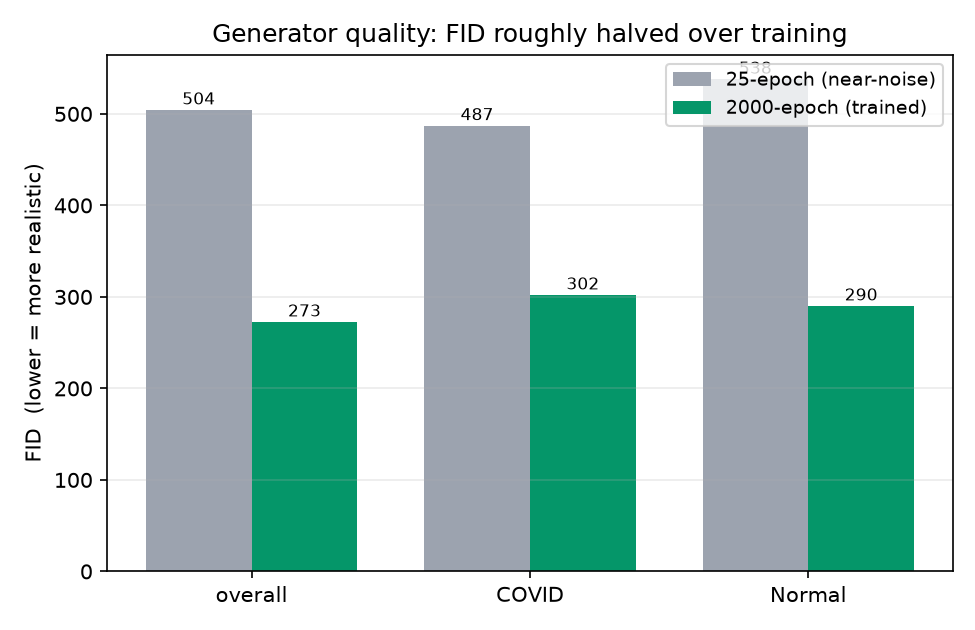
\includegraphics[width=0.78\linewidth]{fid_drop.png}
\caption{FID roughly halved between the 25-epoch and 2000-epoch generators, overall
and per class --- consistent with the generator learning CXR-like structure.}
\end{figure}

\begin{figure}[htbp]
\centering
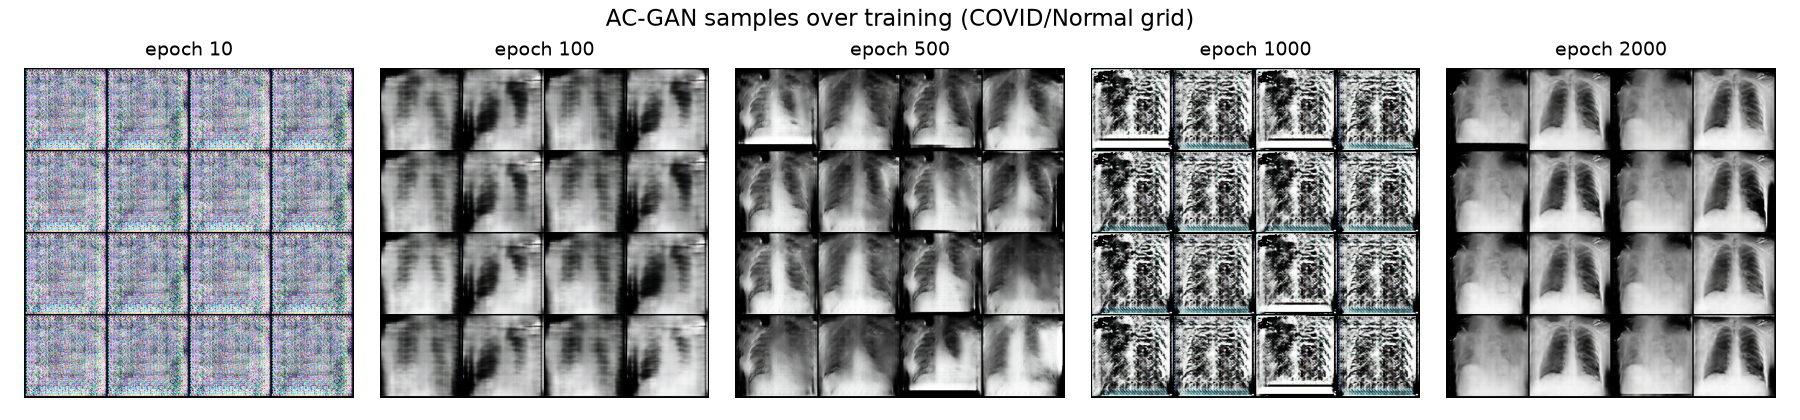
\includegraphics[width=0.78\linewidth]{gan_samples.png}
\caption{AC-GAN samples over training: pure noise at epoch 10 $\rightarrow$
recognizable chest X-rays (visible ribcage and lung fields) by epoch 2000,
consistent with the FID drop.}
\end{figure}

\subsection{Multi-seed check --- is the ``flat'' result just one unlucky run?}
The main table above compares a single CNN-AD run to a single CNN-SA run, and a
0.5-point difference on 192 images is one test image, so on its own it could be
noise. To check, we retrained the \emph{faithful Stage~1 classifier} (frozen VGG16,
plain head --- no Stage~2 changes) from scratch for 3 seeds in both modes
(\code{stage1\_multiseed.py}; summary in \code{runs/stage1\_multiseed/summary.json}).

\begin{table}[htbp]
\centering
\begin{tabular}{@{}lccc@{}}
\toprule
\textbf{Frozen Stage 1, 3 seeds} & \textbf{Accuracy} & \textbf{COVID recall} & \\
\midrule
CNN-AD (real only)   & 91.15\% $\pm$ 0.43 & 89.81\% $\pm$ 0.65 & \\
CNN-SA (+ synthetic) & 91.32\% $\pm$ 0.25 & 87.04\% $\pm$ 1.73 & \\
Augmentation lift    & \textbf{+0.17} & $-$2.78 & \\
\bottomrule
\end{tabular}
\end{table}

\noindent The accuracy lift ($+0.17$) is \emph{smaller than the seed-to-seed
spread} ($\pm$0.3--0.4), i.e.\ statistically indistinguishable from zero --- so
``flat'' is a robust description, not a one-run fluke. If anything COVID recall
drifts slightly \emph{down} ($-2.78$, within a couple of images), the opposite of
the paper's ``augmentation raises COVID recall'' story. Bottom line: in the frozen
Stage~1 model, pooling synthetic data gives \textbf{no reliable accuracy gain}.

\subsection{Combined diagnosis of the two anomalies}
\label{sec:diagnosis}
\begin{itemize}[nosep,leftmargin=1.4em]
  \item \textbf{Anomaly A (high baseline):} the tests \emph{weaken} the two obvious
        shortcut explanations --- cross-source (Test~2) and coarse-global (Test~3).
        The explanation we find most consistent with the evidence is that the
        \textbf{modern Kaggle data is cleaner, larger, and more separable} than the
        paper's 2020 hand-merged set, so our detector is doing legitimate but
        \emph{easier} classification; the gain sits in COVID recall
        (0.69$\to$0.89). We cannot fully rule out a residual dataset artifact
        (Section~\ref{sec:caveat}).
  \item \textbf{Anomaly B (flat augmentation):} FID halved with essentially no
        downstream change (Test~5), which points away from image quality as the
        cause. The explanation we favour is the \textbf{frozen VGG16 head}: with the
        backbone frozen, only $\sim$33K linear params train, so synthetic images can
        only nudge a boundary on top of \emph{fixed} features rather than reshape
        them. The same frozen backbone also limits how much the weak synthetic
        signal (Test~4) can \emph{hurt} --- which is consistent with the observed
        \emph{flat} (neither helping nor hurting) result.
\end{itemize}
\noindent This reading points directly to Stage~2: if the frozen head is the
blocker, the natural thing to try is to \emph{unfreeze some capacity where
augmentation could act} --- which is exactly what we test next. (This is a
hypothesis to test, not a settled conclusion; Section~5 checks whether it holds.)

\subsection{Open caveat}
\label{sec:caveat}
Test~3 argues against a \emph{coarse} shortcut but cannot rule out a
\textbf{fine-scale, dataset-specific artifact} (a rescaling-kernel signature,
JPEG/compression fingerprint, or faint watermark). Such an artifact would live in
fine detail, would \emph{also} vanish under downsampling, and so would look just
like detail-dependence in the Test~3 table. We flag this as the main open question
about anomaly~A; how it could be settled is discussed under future work
(Section~\ref{sec:discussion}).

\subsection{How the models were run}
The GAN was trained for the paper's full \textbf{2000 epochs} (batch 64,
Adam \code{lr=2e-4}, $\beta_1=0.5$), which took roughly \textbf{18 hours} on an
Apple-silicon GPU (MPS), checkpointing every 100 epochs so the run is
interruption-safe; the epoch-2000 generator is saved at
\code{weights/covidgan\_generator\_final.pt}. Each detector (CNN-AD / CNN-SA)
trains in about a minute on the same hardware. The pipeline also runs on a free
Colab GPU.

% =====================================================================
\section{Improved architecture (Stage 2)}
% =====================================================================

All Stage~2 code is in the separate \code{stage2/} package; the Stage~1 code is
unchanged and only imported for its data/metrics utilities. Stage~1 surfaced
\emph{two} distinct bottlenecks, so we improve the architecture on two fronts:

\begin{itemize}[nosep,leftmargin=1.4em]
  \item \textbf{Track~A --- the classifier} (anomaly~B, the frozen head): unfreeze
        the encoder so augmentation has something to act on
        (Section~\ref{sec:trackA}).
  \item \textbf{Track~B --- the generator} (the weak synthetic signal of Test~4):
        fix the parts of the GAN that suppress diversity and encourage a
        pathology-free ``label fingerprint'' (Section~\ref{sec:trackB}).
\end{itemize}

All the changes are drawn from the assignment's list of allowed modifications
(``change the encoder,'' ``add normalization layers,'' ``improve the generator /
discriminator,'' ``add regularization,'' ``change the latent dimension'').

\subsection{Track A --- fine-tune the classifier encoder}
\label{sec:trackA}
Two coupled changes to the detector, addressing the Stage~1 diagnosis
(Section~\ref{sec:diagnosis}):

\begin{table}[htbp]
\centering\small
\begin{tabular}{@{}clp{3.2cm}l@{}}
\toprule
\# & \textbf{Change} & \textbf{Assignment category} & \textbf{Where} \\
\midrule
1 & Unfreeze the top VGG16 conv block(s) --- domain fine-tuning of the encoder & ``Change the encoder'' & \code{stage2/model.py} \\
2 & Add BatchNorm to the head (Dense(64) $\rightarrow$ BatchNorm1d $\rightarrow$ ReLU $\rightarrow$ Dropout $\rightarrow$ Dense(2)) & ``Add normalization layers'' & \code{stage2/model.py} \\
\bottomrule
\end{tabular}
\end{table}

Trained with \textbf{discriminative learning rates} --- fresh head at
$1\mathrm{e}{-3}$, unfrozen pretrained backbone at $1\mathrm{e}{-5}$ --- so
ImageNet filters are gently adapted, not destroyed on $\sim$900 images. We report
\textbf{two variants} to show the effect of how much encoder capacity we unlock:

\begin{table}[htbp]
\centering
\begin{tabular}{@{}lcc@{}}
\toprule
\textbf{Variant} & \textbf{Top blocks fine-tuned} & \textbf{Trainable params} \\
\midrule
Stage 1 (baseline) & 0 (frozen) & 33K \\
Stage 2 / uf=1 & 1 & 7.11M \\
Stage 2 / uf=2 & 2 & 13.01M \\
\bottomrule
\end{tabular}
\end{table}

\paragraph{Why we expected improvement.} This follows from the Stage~1 analysis
rather than being an arbitrary tweak. Stage~1 pointed to the frozen head as the
likely blocker (FID halved yet CNN-SA did not move). Unfreezing the top block(s)
should (a)~let the encoder adapt ImageNet features to CXR texture --- which we
expect to raise the baseline --- and (b)~make the features \emph{trainable}, so
synthetic data can reshape them and the augmentation effect can reappear. Both are
predictions to be checked, not foregone conclusions; we test them next.

\subsection{Track B --- improve the generator}
\label{sec:trackB}
Track~A gives the classifier capacity to \emph{use} good synthetic data, but
Test~4 showed the synthetic data itself is weak --- it carries little transferable
pathology. Reading the Stage~1 generator code turned up concrete, likely reasons,
which motivate a set of standard GAN fixes.

\paragraph{What is wrong with the Stage 1 generator.}
\begin{itemize}[nosep,leftmargin=1.4em]
  \item \textbf{The noise is nearly switched off.} Stage~1 samples the latent as
        $z \sim \mathcal{N}(0, 0.02)$ (\code{covidgan/models.py}, \code{sample\_z}).
        With a std of $0.02$ the noise vector barely varies, so the generator's
        output is driven almost entirely by the \emph{class label}, not by $z$.
        That crushes sample diversity (a direct cause of the high FID) and makes
        the class the dominant axis of variation --- exactly the ``label
        fingerprint'' Test~4 detected. Notably $0.02$ is the classic DCGAN
        \emph{weight-initialisation} std, so this looks like a reconstruction slip
        (an init constant applied to the noise). The standard choice is
        $z \sim \mathcal{N}(0,1)$.
  \item \textbf{The AC-GAN objective rewards that fingerprint.} The auxiliary
        class head lets the generator satisfy its class loss by stamping an easy,
        separable marker rather than learning real COVID/Normal pathology.
  \item \textbf{No small-data regularisation.} With only 403 COVID images the
        discriminator overfits within a few epochs, starving the generator of a
        useful gradient.
\end{itemize}

\paragraph{The changes (\code{stage2/gan\_improved.py}, \code{train\_gan\_improved.py}).}
\begin{table}[htbp]
\centering\small
\begin{tabular}{@{}clp{3.4cm}l@{}}
\toprule
\# & \textbf{Change} & \textbf{Assignment category} & \textbf{Targets} \\
\midrule
3 & Latent noise $z\sim\mathcal{N}(0,0.02)\to\mathcal{N}(0,1)$ & ``change the latent dimension'' & diversity / fingerprint \\
4 & \textbf{DiffAugment} on D's real+fake inputs & ``add regularization'' & small-data overfitting \\
5 & \textbf{Spectral-norm} discriminator, DCGAN weight init & ``improve the discriminator'' & training stability \\
\bottomrule
\end{tabular}
\end{table}

The architecture (layer shapes, $\sim$22M G / $\sim$2M D params) is otherwise
unchanged, so any improvement is attributable to the training recipe, not a bigger
model. We deliberately kept the AC-GAN objective for a controlled comparison; a
projection discriminator (which removes the auxiliary-classifier fingerprint at its
root) is noted as a further step in Section~\ref{sec:discussion}.

\paragraph{Why we expected improvement, and how we test it.} Restoring the noise
scale should raise diversity (lower FID) and dilute the label fingerprint;
DiffAugment should let the small-data discriminator keep giving a useful signal.
We evaluate on \emph{both} axes: FID (realism/diversity of the generator) and the
downstream CNN-SA lift when the improved synthetic pool augments the \emph{Track~A}
(trainable-encoder) classifier --- the setting where, unlike the frozen Stage~1
model, better data can actually be used. We are explicit that these are
predictions: Test~5 already showed that \emph{quality alone} need not move the
downstream number, so an FID drop is necessary but may not be sufficient.

% =====================================================================
\section{Improved results (Stage 2)}
% =====================================================================

Same 192-image real test set throughout, so all rows are comparable.

\subsection{Main result --- paper / reconstruction / improved}
\label{sec:mainresult}
Stage~2 rows are \textbf{mean $\pm$ std over 5 seeds} (\code{stage2/multiseed.py},
with the seed-level numbers in \code{stage2/results/multiseed\_uf1.json} and
\code{multiseed\_uf2.json}); paper and Stage~1 are single runs.

\begin{table}[htbp]
\centering\small
\begin{tabular}{@{}lccc@{}}
\toprule
\textbf{Model} & \textbf{CNN-AD (real only)} & \textbf{CNN-SA (+ synthetic)} & \textbf{Aug.\ lift} \\
\midrule
Paper (Waheed et al.\ 2020) & 85.00\% & 95.00\% & +10.00 \\
Stage 1 reconstruction (frozen) & 90.62\% & 90.10\% & $-$0.52 (flat) \\
Stage 2 improved / uf=1 (1 blk + BN) & 92.50\% $\pm$ 0.71 & 93.65\% $\pm$ 1.16 & \textbf{+1.15} \\
Stage 2 improved / uf=2 (2 blk + BN) & \textbf{94.48\% $\pm$ 0.97} & \textbf{96.67\% $\pm$ 0.71} & \textbf{+2.19} \\
\bottomrule
\end{tabular}
\end{table}

COVID recall (where the gap lives):

\begin{table}[htbp]
\centering
\begin{tabular}{@{}lccc@{}}
\toprule
\textbf{Model} & \textbf{CNN-AD} & \textbf{CNN-SA} & \textbf{Recall lift} \\
\midrule
Stage 2 / uf=1 & 88.89\% $\pm$ 1.76 & 91.39\% $\pm$ 1.62 & +2.50 \\
Stage 2 / uf=2 & 93.33\% $\pm$ 3.22 & 96.67\% $\pm$ 2.08 & +3.33 \\
\bottomrule
\end{tabular}
\end{table}

\noindent\textbf{Both predictions are borne out} in these runs: the baseline rose
(90.6$\to$94.5\%) \emph{and} augmentation now helps rather than being flat. At
uf=2, \textbf{CNN-SA (96.67\%) edges past the paper's 95\%}. We state this as a
5-seed result with the spreads shown, not as a single lucky run.

\begin{figure}[htbp]
\centering
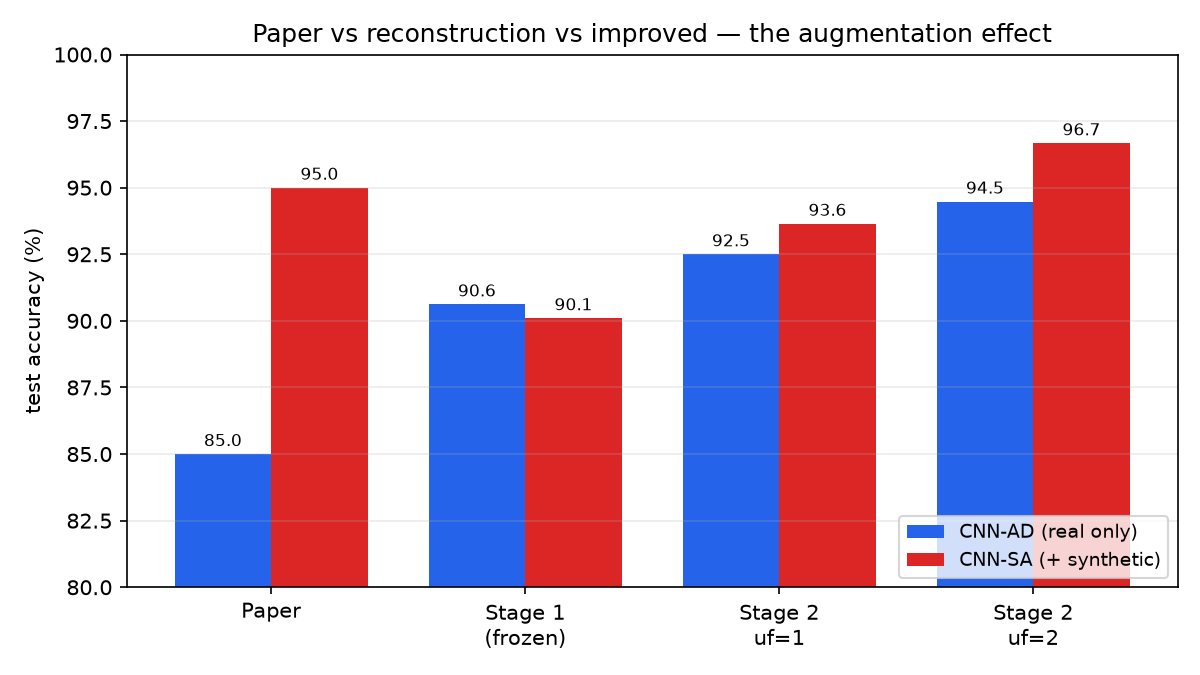
\includegraphics[width=0.82\linewidth]{comparison_bar.png}
\caption{Paper vs reconstruction vs improved --- CNN-AD (real only) vs CNN-SA
(+synthetic). Stage~1 (frozen) shows no augmentation gain; both Stage~2 variants
raise the baseline and restore a positive lift, with uf=2 CNN-SA edging past the
paper's 95\%.}
\end{figure}

\subsection{Test 6 --- Multi-seed robustness + capacity ablation}
\begin{itemize}[nosep,leftmargin=1.4em]
  \item \textbf{Hypothesis:} a single-run ``+1.5 points'' could be seed noise; and
        more unlocked capacity should give more room for augmentation.
  \item \textbf{Method:} retrain both arms from scratch for \textbf{5 seeds} each,
        at uf=1 and uf=2 (\code{stage2/multiseed.py}). The full per-seed results are
        the numbers in the Section~\ref{sec:mainresult} tables (mean $\pm$ std),
        with raw values in \code{stage2/results/multiseed\_uf\{1,2\}.json}.
  \item \textbf{Result:} the lift held across all 5 seeds (uf=2: +2.19 acc,
        +3.33 recall), and the COVID-recall lift is \textbf{larger than each arm's
        seed-to-seed spread} --- so it is unlikely to be pure seed noise. uf=2 beat
        uf=1 on both baseline and lift.
  \item \textbf{Verdict:} within this setup the augmentation effect looks robust to
        seed choice, and the amount of unlocked encoder capacity appears to control
        its size (uf=2 $>$ uf=1). We report it as a consistent 5-seed effect, not a
        formal significance test.
\end{itemize}

\subsection{Test 7 --- Data-scarcity curve (why is our lift smaller than +10?)}
\begin{itemize}[nosep,leftmargin=1.4em]
  \item \textbf{Hypothesis:} our full-data lift ($\sim$+2) is smaller than the
        paper's +10 because our baseline is near ceiling; the paper's +10 came from
        a \textbf{data-starved 85\%}. Augmentation should therefore help \emph{more}
        as real data shrinks.
  \item \textbf{Method:} subsample the \textbf{real} training set (stratified) to
        10/25/50/100\% while keeping the \textbf{full} synthetic pool fixed;
        compare CNN-AD vs CNN-SA at each fraction (uf=2, 3 seeds;
        \code{stage2/data\_scarcity.py}).
\end{itemize}

\begin{table}[htbp]
\centering
\begin{tabular}{@{}lccccc@{}}
\toprule
\textbf{real frac} & \textbf{n\_real} & \textbf{CNN-AD} & \textbf{CNN-SA} & \textbf{acc lift} & \textbf{recall lift} \\
\midrule
0.10 & 93  & 86.98\% & 89.24\% & +2.26 & +1.39 \\
0.25 & 233 & 89.58\% & 92.88\% & \textbf{+3.30} & +4.63 \\
0.50 & 466 & 91.32\% & 93.06\% & +1.74 & +0.93 \\
1.00 & 932 & 93.92\% & 96.01\% & +2.08 & +1.39 \\
\bottomrule
\end{tabular}
\end{table}

\begin{figure}[htbp]
\centering
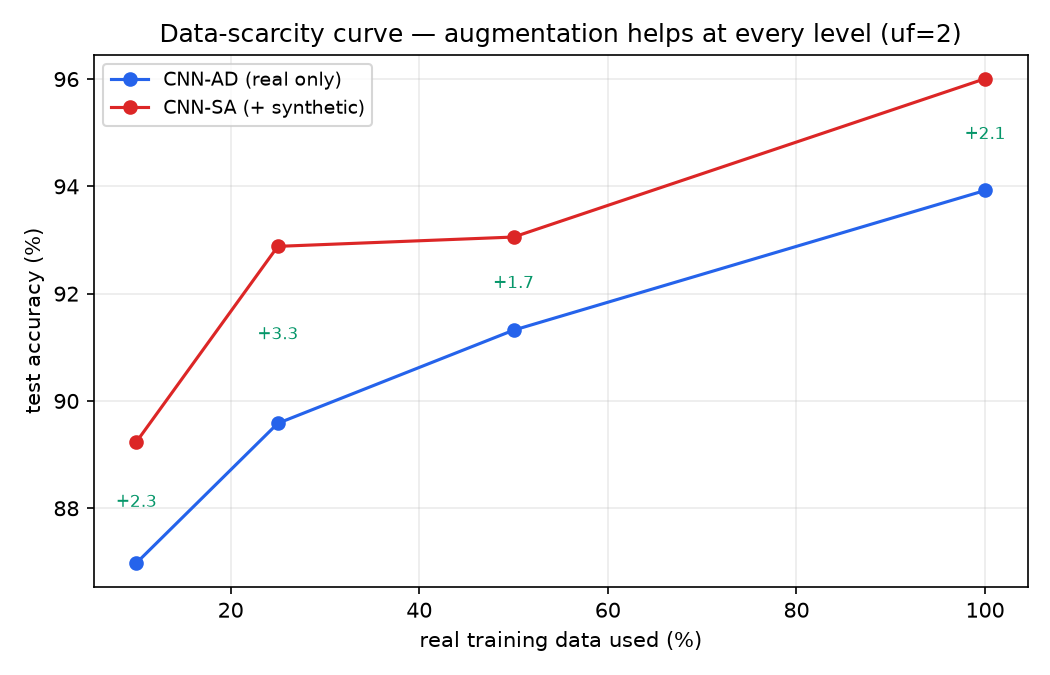
\includegraphics[width=0.72\linewidth]{data_scarcity.png}
\caption{Data-scarcity curve: CNN-SA (red) stays above CNN-AD (blue) at every
real-data fraction; the green labels are the accuracy lift.}
\end{figure}

\begin{itemize}[nosep,leftmargin=1.4em]
  \item \textbf{Result:} the baseline degrades monotonically as data shrinks
        (93.9$\to$87.0\%), and augmentation helps at \textbf{every} level (+1.7 to
        +3.3), \textbf{largest in the low-to-mid regime} (peak +3.30 at 25\%).
  \item \textbf{Verdict:} supports the paper's ``augmentation rescues data-starved
        models'' thesis \emph{directionally}. Honest caveat: not perfectly
        monotonic, and the 10\% point is noisy (only 93 images; its 3 seeds ran
        +4.17/$-$1.04/+3.65), so we frame it as ``consistently positive, strongest
        at low-to-mid data,'' not ``monotonic.''
\end{itemize}

\subsection{Test 8 --- Generalization curve (are we overfitting?)}
\begin{itemize}[nosep,leftmargin=1.4em]
  \item \textbf{Hypothesis:} train accuracy hits $\sim$100\% within $\sim$10
        epochs, so maybe the model overfits and we should stop earlier.
  \item \textbf{Method (bias-safe):} the reported models use a \textbf{fixed 15
        epochs chosen test-blind}. Separately, a \emph{diagnostic} run logs
        per-epoch \textbf{test} accuracy (\code{stage2/diagnostic\_curve.py}, 25
        epochs) --- \textbf{for analysis only; not used to select the epoch}, since
        choosing the epoch by test score would be selecting on the test set and
        would bias the result.
  \item \textbf{Result:} train saturates $\geq$99\% by epoch 3--6, yet
        \textbf{test accuracy never degrades} through 25 epochs (AD plateau
        $\approx$93.7\% $\pm$0.76, SA $\approx$96.5\%, drifting slightly up). SA's
        curve sits above AD's at essentially every epoch. The single-epoch
        ``peaks'' (AD 95.83\%@24, SA 97.40\%@6) are random noise spikes at
        different epochs.
\end{itemize}

\begin{figure}[htbp]
\centering
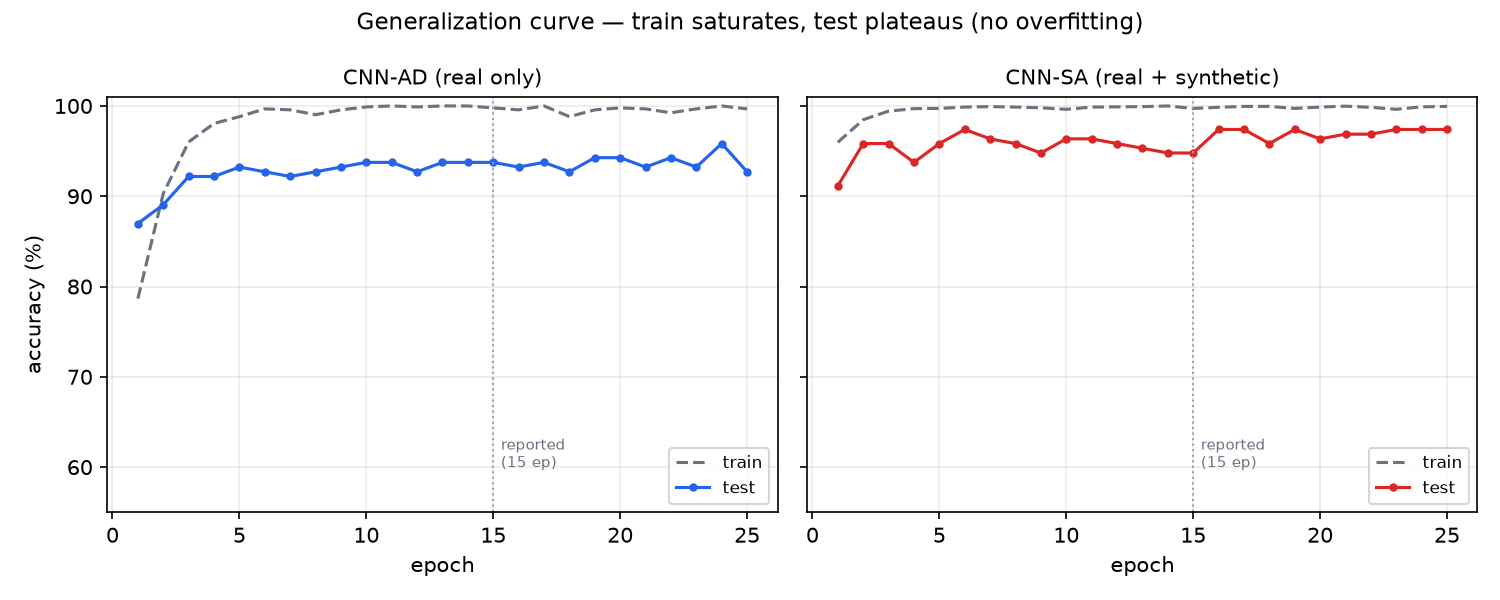
\includegraphics[width=0.72\linewidth]{generalization_curve.png}
\caption{Generalization curve: train accuracy (grey dashed) saturates near 100\%,
but test accuracy (solid) plateaus rather than degrading through 25 epochs; the
fixed 15-epoch mark sits on the plateau. SA's test curve stays above AD's
throughout.}
\end{figure}

\begin{itemize}[nosep,leftmargin=1.4em]
  \item \textbf{Verdict:} we see \textbf{no sign of harmful overfitting} here ---
        train saturation did not translate into test degradation. ``Train longer''
        neither clearly helps nor hurts, and the fixed 15-epoch mark sits on the
        plateau, so early stopping was not needed for a valid result; proper
        \emph{validation}-based early stopping (never on the test set) is a cleaner
        protocol we note for future work. The noise-spike peaks also illustrate
        \emph{why} tuning the epoch on the test set would bias the result.
\end{itemize}

% =====================================================================
\section{Discussion}
\label{sec:discussion}
% =====================================================================

\paragraph{What worked.} Stage~2 behaved in the direction the Stage~1 analysis
predicted: unfreezing the encoder raised the baseline \emph{and} brought back a
positive augmentation effect --- the paper's core finding that our faithful
\emph{frozen} reconstruction had not reproduced. Framing each step as a test
(cross-source, coarse shortcut, image quality, seed noise) let us support or weaken
specific explanations rather than just assert them, even where the tests are not
individually conclusive.

\paragraph{What did not.} We did not reproduce the paper's \textbf{+10-point}
magnitude. The most likely reason is \emph{available headroom} rather than a broken
method: our $\sim$94.5\% baseline on cleaner modern data has little room to gain 10
points, whereas the paper started at 85\%. The data-scarcity curve is consistent
with this reading --- the lift tends to grow as the baseline weakens --- though
that curve is itself noisy at the extreme-scarce end.

\paragraph{What we learned.} Our results are consistent with the CovidGAN
augmentation benefit being \textbf{real but contingent} on (a)~the classifier
having trainable capacity to absorb new data and (b)~the baseline not already being
near ceiling. Freezing the backbone, or starting from an easy high baseline, both
appear to suppress it. Comparing three regimes on identical data --- frozen
(Stage~1), uf=1, uf=2 --- plus the scarcity sweep is what lets us say this with
some confidence.

\paragraph{On the dataset.} We reconstructed on the paper's own cited sources, not
substitutes: the paper merged three public datasets --- Cohen's IEEE
\code{covid-chestxray-dataset}, the Kaggle COVID-19 Radiography Database, and
\code{agchung/Figure1} --- and deduplicated them, with the Normal class coming from
the Kaggle Radiography Database. The main deviation is \emph{version}, not source:
that Kaggle database has been re-released several times since 2020 and is now much
larger and cleaner than the March-2020 snapshot the paper used. This version gap is
our leading explanation for the higher, easier baseline (anomaly~A), and it is not
something we can fully undo, since the authors published no image-level manifest of
their exact 403/721 selection.

\paragraph{Limitations and future work.} Numbers are 5-seed (full data) / 3-seed
(scarcity) means, and the 10\% scarcity point is noisy; a proper significance test
and more seeds there would strengthen the claims. Two concrete next steps:
\begin{itemize}[nosep,leftmargin=1.4em]
  \item \textbf{Independent-dataset validation.} The main open question (anomaly~A,
        Section~\ref{sec:caveat}) is whether the strong baseline reflects real
        transferable pathology or a dataset-specific fine-scale artifact. The way to
        settle it is to evaluate CNN-AD on an \emph{independent} public CXR dataset
        with both classes, non-overlapping with our sources. We did not run this
        (the IEEE set cannot serve --- it is one of the paper's COVID sources and
        has no Normal class --- so a genuinely separate dataset is needed).
  \item \textbf{Validation-based early stopping.} We used a fixed, test-blind epoch
        count; stopping on a held-out \emph{validation} split (never the test set)
        would be a cleaner protocol.
  \item \textbf{Pretrain-then-finetune on the synthetic data.} Rather than
        \emph{pooling} synthetic and real images (what we and the paper do), an
        alternative is to pretrain the (unfrozen) encoder on the synthetic pool to
        pick up CXR-like low-level structure, then finetune on real data ---
        letting the network keep what the generator learned about image structure
        while shedding its spurious class fingerprint (Test~4). This only applies to
        the Stage~2 trainable-encoder setting.
\end{itemize}

% =====================================================================
\section{Reproducing the results}
% =====================================================================

\noindent\textbf{Stage 1 (reconstruction).}
\begin{lstlisting}[language=bash]
# 1. Train CovidGAN (generator + discriminator), paper's 2000 epochs
python train_gan.py --manifest data/manifest.csv --out-dir runs/gan
# 2. Sample the trained generator into the synthetic augmentation pool
python generate_synthetic.py --checkpoint runs/gan/checkpoints/covidgan_final.pt \
    --out-dir data/synthetic
# 3. Baseline: CNN on real data only (CNN-AD)
python train_classifier.py --manifest data/manifest.csv --mode ad --out-dir runs/cnn_ad
# 4. Augmented: CNN on real + synthetic (CNN-SA)
python train_classifier.py --manifest data/manifest.csv --mode sa \
    --synthetic-dir data/synthetic --out-dir runs/cnn_sa
# FID (generator quality)
python evaluate_fid.py --real-manifest data/manifest.csv --synthetic-dir data/synthetic
\end{lstlisting}

\noindent\textbf{Stage 2 (improved model).}
\begin{lstlisting}[language=bash]
# improved model, both arms (uf=2 shown; use --unfreeze-blocks 1 for uf=1)
python -m stage2.train_stage2 --mode ad --unfreeze-blocks 2 --out-dir runs/stage2_cnn_ad
python -m stage2.train_stage2 --mode sa --unfreeze-blocks 2 \
    --synthetic-dir data/synthetic --out-dir runs/stage2_cnn_sa
# multi-seed AD-vs-SA (mean +/- std) -- run for uf=1 and uf=2
python -m stage2.multiseed --seeds 0 1 2 3 4 --unfreeze-blocks 1 --out-root runs/stage2_multiseed
python -m stage2.multiseed --seeds 0 1 2 3 4 --unfreeze-blocks 2 --out-root runs/stage2_multiseed_uf2
# supporting analyses
python -m stage2.data_scarcity --fractions 0.1 0.25 0.5 1.0 --seeds 0 1 2 --unfreeze-blocks 2
python -m stage2.diagnostic_curve --unfreeze-blocks 2 --epochs 25   # diagnostic only
# assemble the paper / reconstruction / improved table
python -m stage2.compare_results
\end{lstlisting}

\noindent Ablations: \code{--unfreeze-blocks \{0..5\}} (0 = Stage~1 behaviour + BN
head); \code{--no-head-bn} drops the BatchNorm.

\FloatBarrier % flush every pending figure/table before the reference list

% =====================================================================
\section{References}
% =====================================================================
\begin{enumerate}[nosep,leftmargin=1.6em]
  \item A.~Waheed, M.~Goyal, D.~Gupta, A.~Khanna, F.~Al-Turjman, P.~R.~Pinheiro,
        ``CovidGAN: Data Augmentation Using Auxiliary Classifier GAN for Improved
        Covid-19 Detection,'' \emph{IEEE Access}, vol.~8, pp.~91916--91923, 2020.
  \item A.~Odena, C.~Olah, J.~Shlens, ``Conditional Image Synthesis with Auxiliary
        Classifier GANs,'' \emph{ICML}, 2017.
  \item K.~Simonyan, A.~Zisserman, ``Very Deep Convolutional Networks for
        Large-Scale Image Recognition'' (VGG16), \emph{ICLR}, 2015.
  \item M.~Heusel, H.~Ramsauer, T.~Unterthiner, B.~Nessler, S.~Hochreiter, ``GANs
        Trained by a Two Time-Scale Update Rule Converge to a Local Nash
        Equilibrium'' (FID), \emph{NeurIPS}, 2017.
  \item T.~Rahman, M.~E.~H.~Chowdhury et al., ``COVID-19 Radiography Database,''
        Kaggle. (Real CXR dataset used for reconstruction.)
  \item J.~P.~Cohen, P.~Morrison, L.~Dao, ``COVID-19 Image Data Collection''
        (ieee8023/covid-chestxray-dataset). (A source of the COVID class.)
\end{enumerate}

\end{document}
